\documentclass{article}

\usepackage[english]{babel}
\usepackage[utf8]{inputenc} \usepackage[T1]{fontenc}

%%%%% 
\usepackage{graphicx} \usepackage{caption} \usepackage{subcaption}

% lock figure into place (H option of \begin{figure})
\usepackage{float}
  
% wrapping text around figures
\usepackage{wrapfig}

\usepackage{setspace}

\usepackage{amsmath}
\usepackage{amssymb}
\usepackage{amsfonts}
\usepackage{amsopn}
\usepackage{braket}
\usepackage{bbm}
\usepackage{dsfont}
\usepackage{kpfonts}
% \usepackage{mathabx}

\parindent=0cm


% Various new commands that ease typesetting math even further
% \newcommand{\assign}{\ensuremath{\coloneq}}
% \newcommand{\rassign}{\ensuremath{\eqcolon}}
\newcommand{\assign}{\ensuremath{:=}}
\newcommand{\rassign}{\ensuremath{=:}}

\newcommand{\of}[1]{\ensuremath{\left( #1 \right)}}
\newcommand{\ofs}[1]{\ensuremath{\left( #1 \right)}}

\newcommand{\norm}[1]{\ensuremath{\| #1 \|}}

\newcommand{\tmop}[1]{\ensuremath{\operatorname{#1}}}

\newcommand{\id}{\ensuremath{\mathds{1}}}
% \newcommand{\id}{\ensuremath{I}}


\newcommand{\conj}[1]{\ensuremath{\overline{#1}}}

\newcommand{\T}{\ensuremath{{}^{\textnormal{T}}}}
\newcommand{\herm}{\ensuremath{{}^{\textnormal{H}}}}

\newcommand{\ft}[1]{\ensuremath{\mathcal{F}\left(#1\right)}}
\newcommand{\ift}[1]{\ensuremath{\mathcal{F}^{-1}\left(#1\right)}}

\newcommand{\fft}[1]{\ensuremath{\mathtt{FFT}\left(#1\right)}}
\newcommand{\ifft}[1]{\ensuremath{\mathtt{IFFT}\left(#1\right)}}

\newcommand{\dotp}[2]{\ensuremath{\langle #1 , #2 \rangle}}

\newcommand{\bigO}[1]{\ensuremath{\mathcal{O}\left( #1 \right)}}

\newcommand{\mat}[1]{\ensuremath{\mathbf{#1}}}

% multi-indices
\newcommand{\mindex}[1]{\ensuremath{\underline{#1}}}

\newcommand{\laplace}{\ensuremath{\operatorname{\Delta}}}

% EOF
  
\usepackage[ruled]{algorithm2e}

% Configure Algorithm2e
\DontPrintSemicolon
\SetKwInOut{Input}{Input}
\SetKwInOut{Output}{Output}

\def\code#1{\texttt{#1}}
\def\classname#1{\textit{#1}}
\def\filename#1{\textit{#1}}

\newtheorem{definition}{Definition}

\begin{document}

\tableofcontents
\clearpage

\section{Basis shape}

A \(D\)-dimensional basis shape \(\mathfrak{K}\)
is a set of \emph{unordered} D-dimensional integer-tuples, also
referred to as \emph{nodes}.  A shape is suitable for our needs if it
satisfies the fundamental property

\begin{equation}
  \label{eq:basis_shape_fundamental_property}
  \mindex{k} \in \mathfrak{K} \Rightarrow \forall
  \mindex{k}-\mindex{e}^d \in \mathfrak{K} \;\forall d \in \{d \;|\;k_d \geq 1\}
\end{equation}

where \(\mindex{e}^d\) is the unit vector in direction \(d\).
That means, if an arbitrary node is part of the basis shape, then all nodes
in the backward cone are part of the shape too.

\subsection{Basis shape description}
To perform a simulation, we do not want to specify every basis shape node
manually. Instead we want a shape that looks like a Hypercube or a Hyperbola.

My program takes the algebraic shape description and converts it into a list of nodes.

\begin{definition}[Surface functions of basis shapes]
  The \(D\) surface functions of an arbitrary \(D\)-dimensional shape are defined by
  \begin{equation}
  s_{\alpha}(\mindex{n})=\max_{k_{\alpha}}
    \left\{\mindex{k} \in \mathfrak{K} \;|\;
      k_d = n_d \; \forall d \neq \alpha
    \right\}
    \label{eq:basis_shape_surface_function}
  \end{equation}
\end{definition}

These functions are well-defined because of the fundamental shape property
(\ref{eq:basis_shape_fundamental_property}).

\begin{definition}[Minimum bounding box of basis shapes]
  The minimum bounding box describes the smallest
  box within which all shape nodes lie.
  \begin{equation}
    L_{\alpha}=\max_{k_{\alpha}}\left\{\mindex{k} \in \mathfrak{K}\right\}
    \label{eq:basis_shape_bbox}
  \end{equation}
\end{definition}

\begin{figure}[H]
  \centering
  \begin{subfigure}[]{0.4\textwidth}
    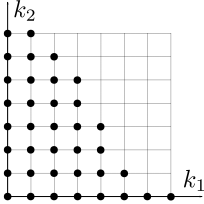
\includegraphics[width=1.0\textwidth]{shape_example}
    \label{fig:shape_example}
  \end{subfigure}
  ~
  \begin{subfigure}[]{0.5\textwidth}
    \begin{tabular}{|| c | c || c | c ||}
      \(\mindex{n}\) & \(s_1(\mindex{n})\) & \(\mindex{n}\) & \(s_2(\mindex{n})\) \\
      (?, 0) & 7 & (0, ?) & 7 \\
      (?, 1) & 5 & (1, ?) & 7 \\
      (?, 2) & 4 & (2, ?) & 6 \\
      (?, 3) & 4 & (3, ?) & 5 \\
      (?, 4) & 3 & (4, ?) & 3 \\
      (?, 5) & 3 & (5, ?) & 1 \\
      (?, 6) & 2 & (6, ?) & 0 \\
      (?, 7) & 1 & (7, ?) & 0 \\
      (?, 8) & \(-\infty\) & (8, ?) & \(-\infty\) \\
    \end{tabular}
  \end{subfigure}
  \caption{Example of a surface description of an 2-dimensional basis shape.}
\end{figure}

\subsection{Common basis shapes}
\begin{definition}[Hypercubic basis shape]
  Given the limits \(\mindex{K} \in \mathbb{N}^D\), a hypercubic shape is defined by

  \begin{equation}
    \label{eq:hypercubic_shape}
    \mathfrak{K}(D,\mindex{K}):=\left\{(k_1,\dots,k_D) \in \mathbb{N}_0^D \;|\; k_d < K_d \forall d\right\}
  \end{equation}
\end{definition}

We derive the surface functions by inserting (\ref{eq:hypercubic_shape}) into
equation
(\ref{eq:basis_shape_surface_function}).
\[
  s_{\alpha}(\mindex{n})=\max_{k_{\alpha}}\left\{(k_{\alpha}<K_{\alpha}) \;\land\;
    (n_d < K_d \;\forall d \neq \alpha)\right\}
\]

\begin{equation}
  s_{\alpha}(\mindex{n})=
  \begin{cases}
    K_{\alpha}-1 & n_d < K_d \;\forall d \neq \alpha \\
    -\infty & otherwise \\
  \end{cases}
\end{equation}

We retrieve the minimum bounding box by inserting (\ref{eq:hypercubic_shape}) into
equation
(\ref{eq:basis_shape_bbox}).

\[
L_{\alpha}=\max_{k_{\alpha}}\left\{k_{\alpha}<K_{\alpha}\right\}
\]

\begin{equation}
L_{\alpha}=K_{\alpha}-1
\end{equation}

\begin{definition}[Hyperbolic cut basis shape]
  Given the sparsity parameter \(S\), a hyperbolic cut shape is defined by
  \begin{equation}
    \mathfrak{K}(D,S):=\left\{(k_1,\dots,k_D) \in \mathbb{N}_0^D \;|\;\prod_{d=1}^D(k_d+1) \leq S\right\}
    \label{eq:hyperbolic_cut_shape}
  \end{equation}
\end{definition}

We derive the surface functions by inserting (\ref{eq:hyperbolic_cut_shape}) into
equation (\ref{eq:basis_shape_surface_function}).

\[
  s_{\alpha}(\mindex{n})=
  \max_{k_{\alpha}}\left\{(k_{\alpha}+1)\prod_{d \neq \alpha} (n_d+1) \leq S \right\} =
  \max_{k_{\alpha}}\left\{k_{\alpha}+1 \leq \frac{S}{\prod_{d \neq \alpha}(n_d+1)}\right\}
\]

\begin{equation}
s_{\alpha}(\mindex{n})=\frac{1}{\prod_{d \neq \alpha} (n_d+1)}-1
\end{equation}

We retrieve the minimum bounding box by inserting (\ref{eq:hyperbolic_cut_shape}) into
equation (\ref{eq:basis_shape_bbox}).

\[
  L_{\alpha}=\max_{k_{\alpha}}\left\{\prod_d(k_d+1) \leq S\right\} =
  \max_{k_{\alpha}}\left\{k_{\alpha}+1 \leq \frac{S}{\prod_{d \neq \alpha}(k_d+1)}\right\}
\]

\begin{equation}
L_{\alpha}=S-1
\end{equation}

\begin{definition}[Shape intersection]
  The intersection of the shapes \(\mathfrak{K}^{A}\) and \(\mathfrak{K}^{B}\) is defined by
  \begin{equation}
    \label{eq:basis_shape_intersection}
    \mathfrak{K}^{A \cap B}=\left\{\mindex{k} \;|\; \mindex{k} \in \mathfrak{K}^A \land
      \mindex{k} \in \mathfrak{K}^B
    \right\}
  \end{equation}
\end{definition}

Using equation (\ref{eq:basis_shape_surface_function}) and (\ref{eq:basis_shape_bbox})
one obtains the surface functions

\begin{equation}
  s_{\alpha}^{A \cap B}(\mindex{n}) = \min\{s_{\alpha}^A(\mindex{n}), s_{\alpha}^B(\mindex{n})\}
\end{equation}

and the minimum bounding box

\begin{equation}
  L_{\alpha}^{A \cap B} = \min\{L_{\alpha}^{A}, L_{\alpha}^{B}\}
\end{equation}

Remark: The \emph{limited hyperbolic cut shape} is an intersection of an
\emph{hypercubic shape} and a \emph{hyperbolic cut shape}.

\begin{definition}[Shape union]
  The union of the shapes \(\mathfrak{K}^{A}\) and \(\mathfrak{K}^{B}\) is defined by
  \begin{equation}
    \label{eq:basis_shape_intersection}
    \mathfrak{K}^{A \cup B}=\left\{\mindex{k} \;|\; \mindex{k} \in \mathfrak{K}^A \lor
      \mindex{k} \in \mathfrak{K}^B
    \right\}
  \end{equation}
\end{definition}

Using equation (\ref{eq:basis_shape_surface_function}) and (\ref{eq:basis_shape_bbox})
one obtains the surface functions

\begin{equation}
  s_{\alpha}^{A \cup B}(\mindex{n}) = \max\{s_{\alpha}^A(\mindex{n}), s_{\alpha}^B(\mindex{n})\}
\end{equation}

and the minimum bounding box

\begin{equation}
  L_{\alpha}^{A \cup B} = \max\{L_{\alpha}^{A}, L_{\alpha}^{B}\}
\end{equation}

\subsection{Basis shape slicing} \label{sec:basis_shape_slice}
Many algorithms, notable the evaluation of a \emph{Hagedorn wavepacket},
use recursive formulas in the form
\( c_{\mindex{k}} = f(c_{\mindex{k}-\mindex{e}^1}, \ldots,
c_{\mindex{k}-\mindex{e}^D}) \)
where \( c_{\mindex{k}} \)
is a value associated with the node \( \mindex{k} \)
and where \( \mindex{e}^d \)
is the unit vector in direction \( d \).
Thus it is beneficial to organize a shape into slices in the following way:

\begin{definition}[Basis shape slice]
  \label{eq:basis_shape_slice}
  Basis shapes \(\mathfrak{K}\) are divided into disjoint slices \(\mathfrak{S}\)
  \begin{equation}
    \mathfrak{K}=\bigcup_{s=0}^{\infty} \left(\mathfrak{S}_s\right)
  \end{equation}
  
  The \( s \)-th
  slice \( \mathfrak{S}^s \) of a shape \( \mathfrak{K} \)
  contains all nodes \( \mindex{k} \in \mathfrak{K} \)
  that satisfy
  \begin{equation}
    \sum_{d=1}^{D} k_d = s
  \end{equation}
  Apparently, \(s\) is the Manhattan distance to the origin.
\end{definition}

\begin{figure}[H]
  \centering
  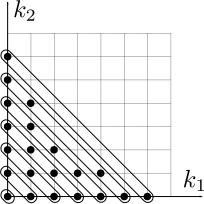
\includegraphics[]{shape_slicing}
  \caption{A basis shape and its slicing.}
\end{figure}


\subsection{Basis shape enumeration}
A basis shape just tells you whether it contains a specific node. But
for many algorithms, one needs to associate values \(c_{\mindex{k}}\) with shape
nodes \(\mindex{k}\). One way to do that is using a dictionary. But it is simpler to
enumerate all nodes in a shape.  This way one is able to keep those
values in an array, ordered according to the enumeration.

\begin{definition}
  A shape enumeration is a (bijective) mapping that orders all nodes
  of \( \mathfrak{K} \)
  and assigns the \(i\)-th node the ordinal \(i\).
\end{definition}

Remark: Due to the close relationship of the enumeration to the shape,
the symbol \(\mathfrak{K}\) is used for both shape and
shape enumeration in this report.

\subsubsection{Data structure}

The data structure is as followes

\begin{verbatim}
template<dim_t D, class MultiIndex>
struct ShapeEnum {
    std::vector< ShapeSlice<D,MultiIndex> > slices;
};
\end{verbatim}

\begin{verbatim}
template<dim_t D, class MultiIndex>
struct ShapeSlice {
    std::size_t offset;
    std::vector< MultiIndex > table;
};
\end{verbatim}

The class \classname{ShapeEnum} (representing \(\mathfrak{K}\)) contains a list
of all non-empty shape slices. The class \classname{ShapeSlice}
\(\mathfrak{S}_s\) contains an array of all nodes \(k \in \mathfrak{S}_s\).

All multi-indices of a slice are lexicographically ordered.
The lexicographical order begins on the first index, continues on the second index and so forth.
\begin{equation}
  \label{eq:lexical_order}
  a_1a_2\dots a_D <_{lex}b_1b_2\dots b_D \iff 
  \begin{cases}
    (a_1 < b_1) \lor (a_1 = b_1 \land a_2\dots a_D <_{lex} b_2\dots b_D) & D > 1 \\
    (d_1 < b_1) & D = 1 \\
  \end{cases}
\end{equation}

\subsubsection{Queries}
The two main operations of a shape enumeration are:
\begin{description}
\item[Retrieve the multi-index \(k\) associated with an given ordinal \(i\)]\mbox{}
  \par
  All multi-indices of a shape are stored in an array.
  Thus we simply return the \(i\)-th multi-index.
\item[Find the ordinal \(i\) of a given multi-index \(k\)]\mbox{}
  \par
  First you have to determine to which slice the multi-index \(k\) belongs by
  \(s = \sum_{d=1}^D \mindex{k}_d \).\par
  All nodes inside a slice are ordered lexicographically. Therefore
  we determine the position of the node \(\mindex{k}\) inside the slice using \textbf{binary search}.
  The final ordinal is the position of \(\mindex{k}\) inside its slice plus
  the number of nodes in all previous slices.
  
\end{description}

\subsubsection{Finding backward neighbours}
A common task is looking up all backward neighbours \(\{k-e^1,\ldots,k-e^D\}\)
of a node \(k\). First all neighbours live inside same slice. Secondly they
are ordered i.e. \(k-e^d\) is stored before \(k-e^{d+1}\). Thirdly due to how lexical order
works, the distance between \((k-e^{d-1})\) and \((k-e^d)\) is usually much larger than
between \((k-e^d)\) and \((k-e^{d+1})\).
The following algorithm takes advantage of this alignment by defining a search range \([a;b]\)
which is the whole slice at the beginning.
After each determined ordinal of the front node, the algorithm subsequently reduces the search range
of the remaining nodes.

\begin{algorithm}[H]
  \caption{Algorithm to find ordinals of backward neighbours}
  \Input{Node \(\mindex{k}\).}
  \Input{Slice that contains the backward neighbours \(\mathfrak{S}\).}
  \Output{Ordinals of backward neighbours \(\{i^1,\ldots,i^D\}\).}
  \(a \leftarrow 1\)\;
  \(b \leftarrow size(\mathfrak{S})\)\;
  \(i^D \leftarrow find(\mindex{k}-\mindex{e}^D) \in \mathfrak{S}[a;b]\)\;
  \(b \leftarrow i^D\)\;
  \For{\(d \leftarrow 1\) \KwTo \(D-1\)}{
    \(i^d \leftarrow find(\mindex{k}-\mindex{e}^d) \in \mathfrak{S}[a;b]\)\;
    \(a \leftarrow i^d\)\;
  }
\end{algorithm}

\subsubsection{Multi-index representation}
The size of a multi-index has a big influence to lookup times and
overall simulation time. Therefore the user can choose at compile-time an appropriate
type to represent multi-indinces. I provide the class \classname{TinyMultiIndex}
that packs the whole multi-index into 64 bits.
Multi-indices of accomplishable simulations should fit into 64 bits.
Otherwise you can define a new multi-index type. A custom implementation
must possess the same semantics as \code{std::array<int,D>}.
Furthermore it has to specialize \code{std::less} that performs lexical index comparison
beginning on the first index.
And it has to specialize \code{std::equal\_to} and \code{std::hash} to
enable use of multi-indices as hashtable keys.

\subsubsection{Alternative data structures}
I tried a hashtable (\code{std::unordered\_set}) to map multi-indices to ordinals.
To represent multi-indices, i used the tiny (64 bits) representation.
These 64 bits can be used unmodified as a hash value.
But queries proved to be 2-3 times slower compared to binary search
despite of \(\mathcal{O}(1)\) compared to \(\mathcal{O}(\log{}n)\) lookup time.
\par
Hashtables are good when querying random keys. But an algorithm working
with basis shapes does \emph{not} access random nodes.
Such algorithms typically access neighbours of previously accessed nodes.
Hashtables map neighbour nodes to seemingly random locations in memory
while an sorted array keeps neighbours together. Thus a hashtable triggers
a lot more cache misses than an sorted array.

\subsubsection{Shape enumeration algorithm}

\begin{figure}[H]
  \centering
  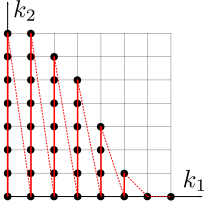
\includegraphics[]{shape_enumerator}
  \caption{Enumerator passage through a 2-dimensional basis shape}
  \label{fig:shape_example}
\end{figure}

The enumerator takes a description of a basis shape and enumerates it in two passes.

In the first pass, knowing the surface functions \(s_{\alpha}\)
and the minimum bounding volume \(L_{\alpha}\) of a shape,
the enumerator iterates through all nodes inside the basis shape in lexicographical order.
Each node is subsequently appended to the proper slice (see section (\ref{sec:basis_shape_slice})).
In the second pass, the enumerator determines the offset (ordinal of first node) of each shape.
The offset is the number of all nodes in previous slices.

\begin{algorithm}[H]
  \emph{Enumerate all nodes in lexicographical order}\;
  \For{\(k_1 \leftarrow 0\) \KwTo \(s_1((0,0,0))\)}{
    \For{\(k_2 \leftarrow 0\) \KwTo \(s_2((k_1,0,0))\)}{
      \For{\(k_3 \leftarrow 0\) \KwTo \(s_3((k_1,k_2,0))\)}{
        \emph{Append lattice node to its slice} \;
        \(\mathfrak{S}_{k_1+k_2+k_3} \leftarrow \mathfrak{S}_{k_1+k_2+k_3} \cdot (k_1,k_2,k_3) \);
      }
    }
  }
  \caption{Enumerator passage through a 3-dimensional basis shape.}
\end{algorithm}

\subsection{Basis shape extension}

\begin{definition}
  Given a basis shape \( \mathfrak{K} \),
  the shape extension \( \overline{\mathfrak{K}} \) is defined by
  \begin{equation}
    \mathfrak{K}_{ext} := \mathfrak{K} \cup 
    \left\{\mindex{k}' \colon \mindex{k}' = \mindex{k} + \mindex{e}^d 
      \forall \mindex{k} \in \mathfrak{K} \forall d\right\}
  \end{equation}
  where \( \mindex{e}^d \) is the unit vector in direction \( d \).
\end{definition}

\begin{figure}[H]
  \begin{center}
    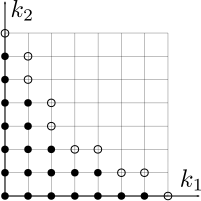
\includegraphics[width=0.5\linewidth]{shape_extension}
  \end{center}
  \caption{Basis shape (filled bullets) and its extension (empty
    bullets)}
\end{figure}

While is possible to define surface functions of the extension,
creating an extended shape this way is impractical.
The basis shape extension is needed when
we have to compute the gradient of a wavepacket. At this stage,
the wavepacket's basis shape is in its enumerated form,
basically just an array of multi-indices. The original shape description is lost.
Therefore we somehow have to create the extension out of the enumerated form.
\par
This task turns out rather straight-forward. We take one slice \(\mathfrak{S}^s\) of
the input basis shape, clone it and
shift it one unit to direction \(d\) by incrementing the \(d\)-th index of each multi-index.
We create one clone for each direction. Then we merge these \(D\) clones and get the
slice \(\mathfrak{S}_{ext}^{s+1}\) of the extended shape. We don't have to sort
during the merging operation.
Notice that nodes inside a clone already are lexicographically ordered.
We just have to interleave the clones in such a way that
lexical order is kept and duplicates get eliminated.
Using a divide and conquer approach, the total algorithmic complexity is
\(\mathcal{O}(D\log{}D \cdot N)\) where \(D\) is the wavepacket dimensionality and \(N\)
is the number of basis shape nodes.

\begin{algorithm}[H]
  \caption{Create extension of an enumerated basis shape.}
  \Input{Enumerated basis shape \(\mathfrak{K}=\bigcup_s\mathfrak{S}^s\)}
  \Output{Basis shape extension \(\mathfrak{K}_{ext}=\bigcup_s\mathfrak{S}_{ext}^s\)}
  \(\mathfrak{S}_{ext}^0 \leftarrow \mindex{0}\)\;
  \ForEach{\(s \leftarrow 1\) \KwTo \(s_{max}+1\)}{
    \For{\(d \leftarrow 1\) \KwTo \(D\)}{
      \(\mathfrak{S}_{ext}^s \leftarrow \mathfrak{S}_{ext}^s \cup
      \left\{\mindex{k}+\mindex{e}^d \;\forall \mindex{k} \in \mathfrak{S}^{s-1}\right\}\)\;
    }
  }
\end{algorithm}

\section{Hagedorn Wavepacket}
\subsection{Scalar Wavepackets}
A \(D\)-dimensional scalar Hagedorn wavepacket is a linear combination of basis functions \(\phi_{\mindex{k}}\)
with coefficients \(c_{\mindex{k}}\)

\begin{equation}
  \label{eq:scalar_hawp_inf}
  \ket{\Phi} := \Phi[\Pi](\vec{x}) = \exp{\left(\frac{iS}{\varepsilon^2}\right)} 
  \sum_{\mindex{k} \in \mathbb{N}^D} c_{\mindex{k}}\phi_{\mindex{k}}[\Pi](\vec{x})
\end{equation}

where \(\varepsilon\) is the semi-classical scaling parameter.\par
Notice that \(\mindex{k}\) is a \emph{multi-index}. It is a tuple that
contains \(D\) integers called indices.
The basis functions \(\Phi_{\mindex{k}}\) are specified by the
Hagedorn parameter set \(\Pi\). It is a tuple
\[
  \Pi := \left(\vec{q},\vec{p},\mat{Q},\mat{P},S\right)
\]
containing the vectors \( \vec{q},\vec{p} \in \mathbb{R}^D \) and
complex matrices \( \mat{Q},\mat{P} \in \mathbb{C}^{D \times D} \). \(S\) is
the global phase.

Equation (\ref{eq:scalar_hawp_inf}) contains infinite many basis functions.
To compute the wavepacket we have to truncate the set of all basis functions to
a finite set \(\mathfrak{K} \subset \mathbb{N}^D\) called \emph{basis shape}.
The wavepacket equation becomes

\[
  \Phi[\Pi](\vec{x}) \approx \exp{\left(\frac{iS}{\varepsilon^2}\right)} 
  \sum_{\mindex{k} \in \mathfrak{K}}c_{\mindex{k}}\phi_{\mindex{k}}[\Pi](\vec{x})
\]

To specify a Hagedorn wavepacket I often use the tuple notation.

\[
  \Phi := \left(\varepsilon,\Pi,\mathfrak{K},c\right)
\]


\subsection{Vectorial Wavepackets}
Vectorial Hagedorn wavepackets \(\Psi\) have multiple components \(\Phi_i\):
\[
  \Psi(\vec{x}) :=
  \begin{pmatrix}
    \Phi_1(\vec{x}) \\
    \Phi_2(\vec{x}) \\
    \vdots \\
    \Phi_N(\vec{x}) \\
  \end{pmatrix}
\]
The components \(\Phi_i\) itself are plain scalar wavepackets.
They have the same scaling parameter \(\varepsilon\) in common but
the Hagedorn parameter set and the basis shape may differ depending on
the concrete type. \\
Common vectorial wavepacket types are:
\begin{description}
\item[Inhomogeneous wavepacket]
  The inhomogeneous wavepacket is the most general case as its components only share
  the scaling parameter \(\varepsilon\).
  \[
    \Phi_i := (\varepsilon, \Pi_i, \mathfrak{K}_i, c_i) \] \[
    \Psi := \left(\varepsilon, 
    \begin{pmatrix}
      (\Pi_1, \mathfrak{K}_1, c_1) \\
      \vdots \\
      (\Pi_N, \mathfrak{K}_N, c_N) \\
    \end{pmatrix}\right)
  \]
\item[Homogeneous wavepackets]
  A homogeneous wavepacket is a special case of the inhomogeneous wavepacket
  since all components share the same Hagedorn parameter set \(\Pi\).
  \[
    \Phi_i := (\varepsilon, \Pi, \mathfrak{K}_i, c_i) \] \[
    \Psi := \left(\varepsilon, \Pi,
    \begin{pmatrix}
      (\mathfrak{K}_1, c_1) \\
      \vdots \\
      (\mathfrak{K}_N, c_N) \\
    \end{pmatrix}\right)
  \]
\item[Gradient]
  The gradient of a scalar Hagedorn wavepacket can be represented using a vectorial Hagedorn
  wavepacket. All components share the same Hagedorn parameter set and the
  same basis shape (which is an extension of the original wavepacket's basis shape).
  \[
    \frac{\partial \Phi}{\partial x_i} := (\varepsilon, \Pi, \mathfrak{K}_{ext}, c'_i) \] \[
    \vec{\nabla} \Phi := \left(\varepsilon, \Pi, \mathfrak{K}_{ext},
    \begin{pmatrix}
      (c'_1) \\
      \vdots \\
      (c'_D) \\
    \end{pmatrix}\right)
  \]
\end{description}


\subsection{Class Diagram}

\begin{figure}[H]
  \centering
  \includegraphics[width=1.0\textwidth]{hawp_inheritance}
  \caption{Wavepacket classes and the inheritance hierarchy}
  \label{fig:hawp_inheritance}
\end{figure}

\subsubsection{Scalar wavepacket classes}

The superclass of all (scalar) Hagedorn wavepackets is \emph{AbstractScalarHaWp}.
It provides read-only access to its parameters through its (abstract) virtual
member functions \emph{eps()}, \emph{parameters()}, \emph{shape()} and \emph{coefficients()}.

It provides following functions as a service:
\begin{description}
\item[evaluate(grid)]
This function gathers the wavepacket parameters \(\varepsilon\), \(\Pi\), \(\mathfrak{K}\) and \(c\) 
through the mentioned virtual member functions \emph{eps()}, \emph{parameters()},
\emph{shape()} and \emph{coefficients()}. Using these parameters it evaluates the wavepacket \(\Phi(\vec{x})\)
on the grid nodes \(\vec{x}\).
\item[evaluate\_basis(grid)]
  It evaluates all basis functions \(\phi_{\mindex{k}}(\vec{x})\) on the grid \(\vec{x}\)
for all \(\mindex{k} \in \mathfrak{K}\). This function is not dependent on the coefficients
\(c_{\mindex{k}}\), therefore I created a further abstract class \emph{AbstractScalarHaWpBasis} that
only contains the parameters \(\varepsilon\), \(\Pi\) and \(\mathfrak{K}\). \emph{AbstractScalarHaWp}
inherits from this base class and extends it with the coefficients \(c_{\mindex{k}}\).
\item[extended\_shape()]
  This non-virtual function returns the basis shape extension \(\mathfrak{K}_{ext}\)
  of the current basis shape \(\mathfrak{K}\). It is used for the gradient computation.
  Creating a basis shape extension is expensive, therefore \(\mathfrak{K}_{ext}\) is cached.
\end{description}

\subsubsection{Vectorial wavepacket classes}
Vectorial wavepacket class are implemented as a composition of scalar wavepackets.
Common aspects are stored in the composition class while different aspects are
stored in the component class.
\par
\emph{Example: } All components of a homogeneous wavepacket share the Hagedorn parameter
set \(\Pi\). Therefore \(\Pi\) is stored inside the composition class \emph{HomogeneousHaWp}.
The component classes \emph{HomogeneousHaWp::Component} only refer to \(\Pi\) to fulfill the contract
of the abstract superclass \emph{AbstractScalarHaWp}.

\subsubsection{Rationale}

\textbf{Abstract superclasses don't provide writeable access to parameters.} \par
Editing parameters of a superclass can have unwanted side-effects
you have no control over since subclasses may share parameters across many wavepackets.
A nice example is an inhomogeneous wavepacket: All components refer to the same Hagedorn parameter set
and scaling parameter \(\varepsilon\).
However concrete subclasses like \emph{ScalarHaWp}, \emph{HomogeneousHaWp}, etc. provide writeable
access to its parameters. This is safe because you know at \emph{compile-time} that you are working with
an homogeneous wavepacket thus you know that if you change the parameter set of one compile, you change
all components. This side-effects are controllable.

\bigskip

\textbf{Scalar and Vectorial wavepackets don't have a common superclass.} \par
The python version actually does that. It proved to be a bad choice.
The problem is that evaluation and parameter access functions would yield
results with different shapes dependent on the actual wavepacket type.
As an example, the function \emph{evaluate()} of a scalar wavepacket yields a scalar value, while
applied on a vectorial wavepacket, this function will yield a vector.
In python this behaviour is halfway manageable because of python's high flexible type system
and numpy's broadcasting operations.
However, dealing with such a behaviour is very hard in C++.
Therefore scalar and vectorial wavepacket don't have a common superclass.

\bigskip

\textbf{There is no dedicated class to represent a gradient of a vectorial wavepacket.} \par
Applying the gradient operator to a vectorial wavepacket is trivial. Just apply it
to its components:
\[\nabla \Psi \equiv
\begin{pmatrix}
  \nabla \Phi_1 \\
  \vdots \\
  \nabla \Phi_N \\
\end{pmatrix}
\]
It is an overkill to introduce a new class, just to replace a for-loop.
Furthermore, storing all coefficients of \(\vec{\nabla}\Psi\) occupies \(\mathcal{O}(D \cdot N \cdot M)\) space.
Using a basis shape of a realistic size \(M=1'000'000\), and wavepacket
dimensionality \(D=10\), one can easily run out of memory.

\subsection{Basis Evaluation}

All basis values are evaluated recursively. Once we have the basis
value at an anchor node \(\mindex{k}\) and the basis values of all
backward neighbours \(\mindex{k}-\mindex{e}^d\), we can compute all
forward neighbours by

\begin{equation}
  \begin{pmatrix}
    \phi_{\mindex{k}+\mindex{e}^1} \\
    \vdots \\
    \phi_{\mindex{k}+\mindex{e}^D}
  \end{pmatrix}
  = \left(
    \sqrt{\frac{2}{\varepsilon^2}} \mat{Q}^\mathrm{-1} (\vec{x}-\vec{q}) \phi_{\mindex{k}}
    - \mat{Q}^\mathrm{H} \mat{Q}^\mathrm{-T}
    \begin{pmatrix}
      \sqrt{k_1} \phi_{\mindex{k}-\mindex{e}^1} \\
      \vdots \\
      \sqrt{k_D} \phi_{\mindex{k}-\mindex{e}^D}
    \end{pmatrix}
  \right)
  \oslash
  \begin{pmatrix}
    \sqrt{k_1+1}\\
    \vdots \\
    \sqrt{k_D+1}
  \end{pmatrix}
\end{equation}

where the operator \(\oslash\) denotes component-wise division.

\begin{figure}[H]
  \centering
  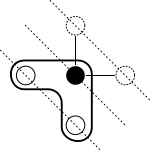
\includegraphics[]{basis_eval_stencil}
  \caption{Stencil of a 2-dimensional wavepacket}
\end{figure}

The root node \(\mindex{0}\) is evaluated by

\begin{equation}
  \label{eq:phi0_Dd}
  \phi_{\mindex{0}}[\Pi]\left(\vec{x}\right)
  \assign
  (\pi\varepsilon^2)^{-\frac{D}{4}} (\det\mat{Q})^{-\frac{1}{2}}
  \exp \left( \frac{i}{2\varepsilon^2}
    \dotp{(\vec{x}-\vec{q})}{\mat{P}\mat{Q}^\mathrm{-1}(\vec{x}-\vec{q})}
    + \frac{i}{\varepsilon^2} \dotp{\vec{p}}{(\vec{x}-\vec{q})}
  \right)
\end{equation}

Basis values of lattice nodes with some negative indices are zero.

\subsubsection{Implementation}
There are many possibilities to implement this recursion scheme. One
possibility is.
\begin{description}
\item[Scatter Type Strategy] We maintains a queue of already computed
  anchor nodes \(\mindex{k}\).  We subsequently remove one feasible(!)
  entry of this queue, compute the basis values of all forward
  neighbours \(\mindex{k}-\mindex{e}^d\) and put those nodes into the
  queue.  To eliminate multiple evaluation of some basis nodes, we
  need to check whether a forward neighbour already has been computed
  using a set.  Therefore the scatter type strategy is very bad suited
  for multi-threading since threads need to synchronize access to this
  set.
\item[Gather Type Strategy] We maintain a queue of not yet computed
  forward neighbours \(\mindex{k}-\mindex{e}^d\). Entries of this queue
  have at least one backward neighbour (called \emph{anchor node})
  that already has been computed.  We subsequently remove one entry of
  the queue (called \emph{child node}) and compute its basis value.
  Then we check, whether \emph{all} backward neighbours of the child
  node are computed. If this is the case put all forward neighbours of
  the child node into he queue.
\end{description}

A straight-forward implementation has at least one of following
difficulties that require complex data structures such as dictionaries
or would require excessive thread synchroniztation if we want
parallelisation:
\begin{description}
\item[A] We need to ensure that an already computed node is a valid
  anchor node (all backward neighbours has been computed too) so that
  we can compute its forward neighbours.
\item[B] We need to avoid multiple evaluation of the same node.
\end{description}

My rather simple solution is to split the shape into splices.  The
\(s\)-th slice contains all nodes \(\mindex{k}\) that fulfill
\( \sum_{d=1}^{D} k_d = s \).

\begin{figure}[H]
  \begin{center}
    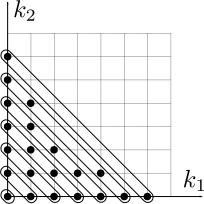
\includegraphics{shape_slicing}
  \end{center}
\end{figure}

Using an \emph{adequate} \footnote{See section \emph{Basis Shape}}
shape, the recusion scheme implies that if we had computed all basis
values of the parent slice \( \mathfrak{K}^{s-1} \) and of the current
slice \( \mathfrak{K}^{s} \), then we can compute all basis values of
the child slice \( \mathfrak{K}^{s+1} \) without having difficulty
\textbf{A}.  Furthermore if we use the gather type strategy where we
iterate through the child slice and compute its basis values, we
automatically avoid difficulty \textbf{B}.

My solution has two compelling advantages:
\begin{description}
\item[Simple data structures] We can keep our computed basis value in
  an array separated slice by slice. We need a \emph{shape
    enumeration} that maps shape nodes to ordinals used as array
  offsets.
\item[Easy parallelisation] I implemented the gather type strategy
  therefore one could simply split the iteration over the child slice
  using \code{pragma omp parallel for}. All previous slices has been
  completely computed therefore the only synchronisation mechanism
  needed is a barrier at the end of the child slice.
\end{description}

\begin{algorithm}[H]
  \Input{number of slices \(S\)}
  \Input{shape enumeration (slices)
    \(\mathfrak{K} = \left(\mathfrak{K}^0, \ldots,
      \mathfrak{K}^{S-1}\right)\)}
  \Output{basis values on each slice
    \(\phi = \left(\phi^0, \ldots, \phi^{S-1}\right)\)} initialization\;
  \(\phi^-, \phi, \phi^+ \gets \emptyset \)\;
 
  \emph{Compute ground state}\;
 
  \( \gets \left\{ \phi_{\mindex{0}}[\Pi](\vec{x}) \right\} \)\;
  \emph{Loop over all slices}\;
  \ForEach{\(\mathfrak{K}^s \in \mathfrak{K}\)}{ \emph{Loop over all
      nodes of next slice}\;
    \For{\(\mindex{k}^{s+1} \in \mathfrak{K}^{s+1}\)}{ \emph{find
        suitable anchor node (in current slice)}\;
      \(\alpha \gets undef \)\\
      \For{\(d \in \{1,\ldots,D\}\)}{ \If{\(k^{s+1}_{d} > 0\)}{
          \(\alpha \gets d\)\; } } \emph{here is our anchor node
        \(\mindex{k}^{s}\)}\;
      \(\mindex{k}^{s} \gets \mindex{k}^{s+1} - \mindex{e}^\alpha\)\;
    
      \emph{compute contribution of anchor node}\;
      \(a \gets
      \frac{\sqrt{2}}{\varepsilon}\left(\mat{Q}^\mathrm{-1}(\vec{x}-\vec{q})\right)_\alpha\phi^{s}_{\mindex{k}}\)
    
      \emph{compute contribution of anchor node's backward
        neighbours}\; \(b \gets 0\)\;
      \For{\(d \in \{1,\ldots,D\}\)}{
        \If{\(k^{s}_{d} > 0\)}{
          \(b \gets b + \sqrt{k^{s}_d}
          \left(\mat{Q}^{\mathrm{H}}\mat{Q}^{\mathrm{-T}}\right)_{\alpha
            d} \phi^{s-1}_{\mindex{k}^{s}-\mindex{e}^d}\)\; } }
    
      \emph{compute value of basis at \(\mindex{k}^{s+1}\)}\;
      \(\phi^{s+1}_{\mindex{k}^{s+1}} \gets
      \frac{a-b}{\sqrt{1+k^{s}_\alpha}} \) } }
  \caption{Recursive basis evaluation of hagedorn wavepacket}
\end{algorithm}

\subsubsection{Algorithmic complexity}
Evaluating \(D\)-dimensional wavepackets involves evaluating \(N\) basis functions \(\phi_k\).
To evaluate a basis function we have to lookup the ordinals of \(D\)
backward neighbours which costs \(\mathcal{O}(D \log{}S)\) because we use binary search.
\(S\) is the size of the largest slice. A shape has at least \(\mathcal{O}(D\log{}N)\)
slices (see hypercubic shape). Therefore
\[
  \mathcal{O}(S)=\mathcal{O}(\frac{N}{D\log{}N}) \approx \mathcal{O}(N)
\]
Gathering values of previous basis functions \(\phi_{k-e^d}\) and computing \(\phi_k\)
has complexity \(\mathcal{O}(D)\).
Thus evaluating all basis functions has complexity
\[
  \mathcal{O}(N \cdot D\log{}S) + \mathcal{O}(N \cdot D) =
  \mathcal{O}(N\log{}^2 N)
\]
when assuming \(D \approx \log{}N\).
Computing the dot-product \(\sum c_k\phi_k\) costs \(\mathcal{O}(N)\)
thus the final \emph{asympotical} complexity
\begin{equation}
  \label{eq:hawp_eval_complexity}
  \mathcal{O}(N\log{}^2N)
\end{equation}

\subsubsection{Evaluating on multiple quadrature points at once}

To evaluate the basis function \(\phi_k\), we need all backward neighbours
\(\phi_k-e^d\).
Unfortunately the program spends much time on looking up the ordinals of these
backward neighbours. To reduce the lookup time vs computation time ratio
I've implemented the possibility to evaluate the basis functions \(\Phi_k\)
on multiple grid nodes at once.

Figure (\ref{fig:hawp_eval_multiqp}) shows the effect of one
evaluation with \(N\) grid nodes compared to \(N\) evaluations with one
grid node each. It shows that the multi-evaluation of a \(10\)-dimensional
wavepacket is up to \(2.5\) times faster than when using single-evaluations.

\begin{figure}[H]
  \centering
  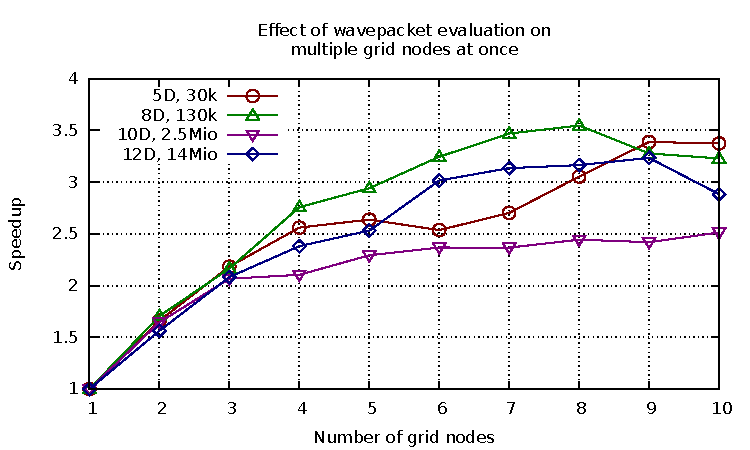
\includegraphics[width=1.0\textwidth]{plots/hawp_eval_multiqp}
  \caption{Effect of multiple quadrature points}
  \label{fig:hawp_eval_multiqp}
\end{figure}

Notice that the benefit of multiple grid nodes is smaller on high dimensions because
lookup time scales with \(\mathcal{O}(D)\) while computation time per basis function
scales with \(\mathcal{O}(D^2)\).

\subsection{Gradient Computation}
Applying the gradient operator to a scalar \(D\)-dimensional Hagedorn Wavepacket 
\( \Phi = \left( \varepsilon, \Pi, \mathfrak{K}, c \right)\)
yields a vectorial Hagedorn Wavepacket \(\Psi=\vec{\nabla}\Phi\) with \(D\) components.
The wavepacket gradient \(\Psi\) has the same parameterset \(\Pi\) as the original wavepacket \(\Phi\),
but has a new coefficients set \(c'\) given by

\begin{equation}
  \label{eq:compute_grad_coeff}
  c'_{\mindex{k}}=c_{\mindex{k}}\vec{p}+\sqrt{\frac{\varepsilon^2}{2}}
  \left(\mat{\overline{P}}
    \begin{pmatrix}
      c_{\mindex{k}+\mindex{e}^1}\sqrt{k_1+1} \\
      \vdots \\
      c_{\mindex{k}+\mindex{e}^D}\sqrt{k_D+1} \\
    \end{pmatrix}
    +\mat{P}
    \begin{pmatrix}
      c_{\mindex{k}-\mindex{e}^1}\sqrt{k_1} \\
      \vdots \\
      c_{\mindex{k}-\mindex{e}^D}\sqrt{k_D} \\
    \end{pmatrix}
  \right)
\end{equation}

Some wavepacket gradient coefficients outside of the original basis shape are non-zero.
Thus the wavepacket gradient needs a new parameter set \(\mathfrak{k}_{ext}\)
with the following property

\begin{equation}
  \label{eq:shape_extension_requirement}
  \mindex{k} \in \mathfrak{K} \Rightarrow
  \left(
     \mindex{k} \in \mathfrak{K}_{ext}
  \right)
  \wedge
  \left(
    \mindex{k}+\mindex{e}^1 \in \mathfrak{K}_{ext}
    \wedge \dots \wedge
    \mindex{k}+\mindex{e}^D \in \mathfrak{K}_{ext}
  \right)
\end{equation}

\subsubsection{How it was done in Python}
The original python code uses a \emph{scatter-type strategy}:
It loops over all \(\mindex{k} \in \mathfrak{K}\) and computes its contribution
to its neighbours in \(\mathfrak{K}_{ext}\). The reason to use this strategy is,
how the shape extension \(\mathfrak{K}_{ext}\) is implemented. It contains far more
entries than required by equation \eqref{eq:shape_extension_requirement}.
Since the scatter-type strategy loops over \(\mathfrak{K}\) and
not over the oversized \(\mathfrak{K}_{ext}\), no computation power is wasted.

\begin{figure}[H]
  \centering
  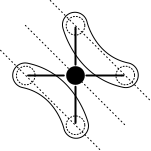
\includegraphics{grad_scatter_stencil}
  \caption{Stencil of scatter-type algorithm}
  \label{fig:grad_scatter_stencil}
\end{figure}

\subsubsection{How I have implemented it}
As my shape extension \(\mathfrak{K}_{ext}\) implementation only contains
nodes that are really required by equation \eqref{eq:shape_extension_requirement},
there is no necessity for me to use the scatter type strategy.
Instead my implementation uses the \emph{gather-type strategy}: It loops over all
\(\mindex{k} \in \mathfrak{K}_{ext}\), gathers the values of its contributors
and finally computes the new coefficients \(c'_{\mindex{k}}\) according to equation
\eqref{eq:compute_grad_coeff}.
I decided to use this strategy because it is much easier to parallelize.
For each node, the program just writes to one instead of \(2D\) locations.
This greatly simplifies parallelization.

\begin{figure}[H]
  \centering
  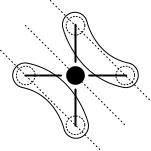
\includegraphics{grad_gather_stencil}
  \caption{Stencil of gather-type algorithm}
  \label{fig:grad_gather_stencil}
\end{figure}

\begin{algorithm}[H]
  \Input{\(\varepsilon\)}
  \Input{wavepacket dimension \(D\)}
  \Input{wavepacket parameters \(\Pi=(\vec{q},\vec{p},\mat{Q},\mat{P}))\)}
  \Input{shape enumeration \(\mathfrak{K}\)}
  \Input{shape extension enumeration \(\mathfrak{K}_{ext}\)}
  \Input{coefficients (scalars) of wavepacket \(\boldsymbol{c}\)}
  \Output{coefficients (\(D\)-dimensional vectors) of wavepacket gradient \(\boldsymbol{\vec{c_\nabla}}\)}
  \For{\(\mindex{k} \in \mathfrak{K}_{ext} \)}{
    \emph{compute contribution of center node}\;
    \(m \leftarrow 0\)\;
    \If{\(\mindex{k} \in \mathfrak{K}\)}{
      \(m \leftarrow c_{\mindex{k}}\)\;
    }

    \emph{compute contribution of backward neighbours}\;
    \(\vec{b} \leftarrow 0\)\;
    \For{\(d \in \{1,\ldots,D\}\)}{
      \If{\(\mindex{k}-\mindex{e}^d \in \mathfrak{K}\)}{
        \(b_d \leftarrow \sqrt{k_d}c_{\mindex{k}-\mindex{e}^d}\)\;
      }
    }

    \emph{compute contribution of forward neighbours}\;
    \(\vec{f} \leftarrow 0\)\;
    \For{\(d \in \{1,\ldots,D\}\)}{
      \If{\(\mindex{k}+\mindex{e}^d \in \mathfrak{K}\)}{
        \(f_d \leftarrow \sqrt{k_d+1}c_{\mindex{k}+\mindex{e}^d}\)\;
      }
    }

    \emph{merge contributions of every node to get the coefficients of the gradient}\;
    \(\vec{c_{\nabla,\mindex{k}}} \leftarrow m\vec{p}+\frac{\varepsilon}{\sqrt{2}}(\mat{\overline{P}}\vec{f}+\mat{P}\vec{b})\)
  }
  \caption{Computes coefficients of the wavepacket gradient \(\vec{\nabla} \Phi\)}
\end{algorithm}

\subsection{Optimized evaluation of vectorial wavepackets}
The naive approach to evaluate vectorial wavepackets, is to separately
evaluate each component. For inhomogeneous wavepackets there is
no better way.
However components of homogeneous wavepackets share the same Hagedorn parameter set
and therefore share some basis functions. How many depends on how large the overlap of
the basis shapes is. Basis shapes of components typically are very similar so
we can benefit if compute shared basis functions only once.

One way to achieve this, is to compute the union of tha
basis shapes of all components:
\[
\mathfrak{K}^{\cup} = \mathfrak{K}^1 \cup \mathfrak{K}^2 \cup \dots \cup \mathfrak{K}^N
\]

Then we compute the basis functions governed by the basis shape union:
\[
\left\{\phi_{\mindex{k}} \;|\;\mindex{k} \in \mathfrak{K}^{\cup}\right\}
\]

Finally, for each wavepacket component \(\Phi_n\),
we compute the dot product of its coefficients \(c_{n,\mindex{k}}\)
with the subset \(\left\{\phi_{\mindex{k}}\;|\; \mindex{k} \in \mathfrak{K}^n\right\}\):

\[
\Phi_n(\vec{x})=\sum_{\mindex{k} \in \mathfrak{K}^n} c_{n,\mindex{k}} \phi_{\mindex{k}}(\vec{x})
\]

Remark: My implementation does the the above computation slice by slice to save memory
the same way as for a scalar wavepacket.

To quantify the improvement, I benchmarked the above algorithm on a homogeneous wavepacket with
varying number of components. All components have the same basis shape which is
the best case for the algorithm (since in this case shapes completely overlap).
The 10-dimensional basis shape had a size of one million nodes.
The results (see figure \ref{fig:hawp_homogen_evaluation_speedup}) show that the
optimized algorithm can be six times faster than perform a naive loop over all
wavepacket components.

\begin{figure}[H]
  \centering
  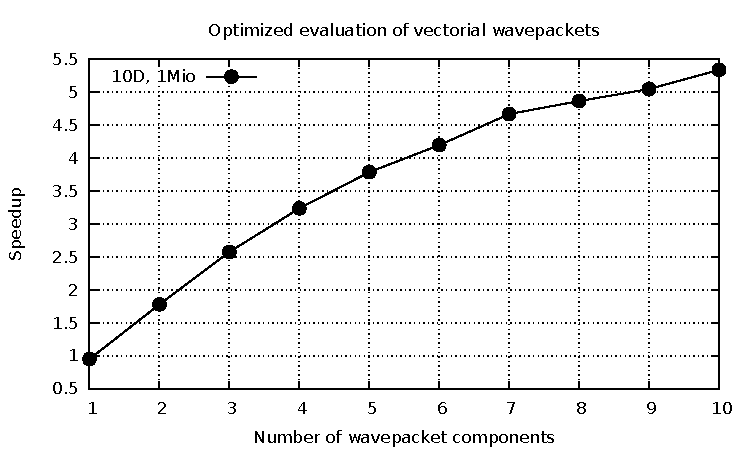
\includegraphics[width=1.0\textwidth]{plots/hawp_eval_homogen_speedup}
  \caption{Archievable speedup compared to naive evaluation.}
  \label{fig:hawp_homogen_evaluation_speedup}
\end{figure}

There is an upper bound to the archievable speedup because the algorithm
avoids multiple evaluation of the same basis functions \(\phi_k\) but does not reduce
time spent on computing the dot-product \(\sum c_k\phi_k\).
Thus when increasing the number of components, computing the dot-product becomes
more and more the bottleneck.

\section{Benchmarks}

\subsection{Wavepacket evaluation}

I benchmarked wavepackets using a hyperbolic cut shape with limits \(100\).
I varied the sparsity between \(2^D\) and \(3^D\) where \(D\) is the wavepacket
dimensionality.

\begin{figure}[H]
  \centering
  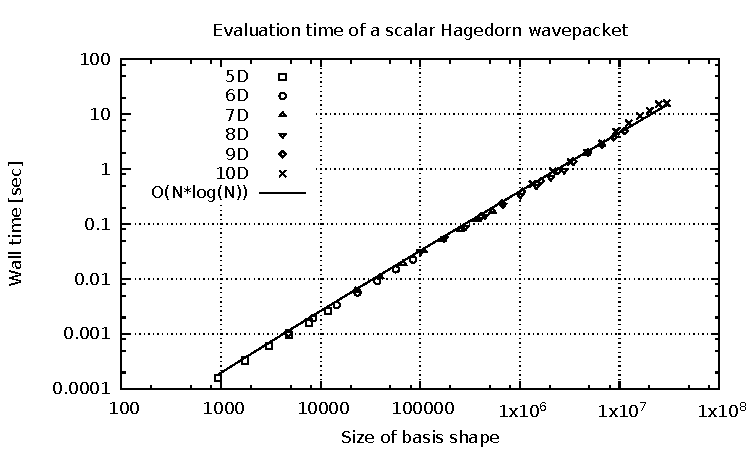
\includegraphics[width=1.0\textwidth]{plots/hawp_eval_benchmark}
  \caption{Time to evaluate a scalar wavepacket}
  \label{fig:hawp_eval_benchmark}
\end{figure}

Evaluating a wavepacket has asymptotical complexity \(\mathcal{O}(D^2N)\) where
\(N\) is number of basis shape nodes.
Since \(D\) corresponds to \(\log{}N\) the asymptotial complexity is \(\mathcal{O}(N\log{}^2N)\)
which seems confirmed by the results which suggest \(\Theta(N\log{}N)\) because asymptotic limit
has not been reached yet.

\begin{figure}[H]
  \centering
  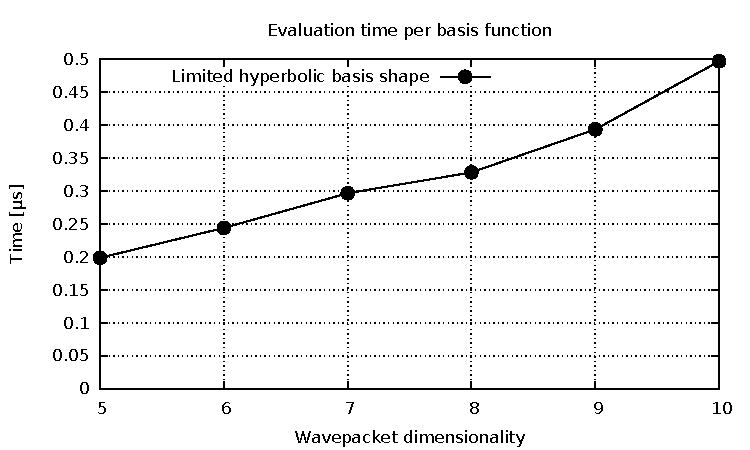
\includegraphics[width=1.0\textwidth]{plots/hawp_eval_efficiency}
  \caption{
    This chart shows the effect of dimensionality to evaluation time.
    It shows the time needed to evaluate one basis function depending
    on dimensionality.
  }
  \label{fig:hawp_eval_efficiency}
\end{figure}

\subsection{Comparison to WaveBlocksND}

\subsubsection{Wavepacket evaluation}

\begin{figure}[H]
  \centering
  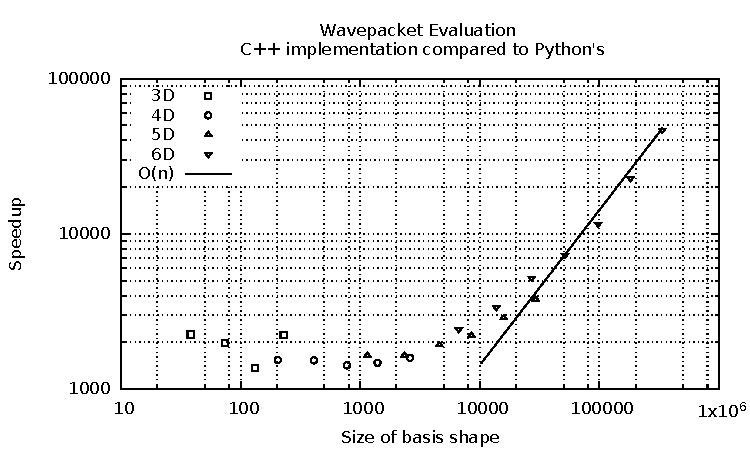
\includegraphics[width=1.0\textwidth]{plots/hawp_eval_cvp_slim}
  \caption{Wavepacket evaluation time in C++ compared to WaveBlocksND.
    WaveBlocksND uses the \textbf{slim recursion} routine.}
  \label{fig:hawp_eval_cvp_slim}
\end{figure}

Apparently, the C++ implementation is asymptotically better than WaveBlocksND by a factor of
\(\mathcal{O}(N)\). My implementation could have slightly better run-time complexity due to slicing but by
no means \(\mathcal{O}(N)\). This implies that run-time complexity of the slim recursion is
quadratical to the basis shape size.
This behaviour is caused by a flaw somewhere inside the slim recursion.
Due to this discovery, I've done all further benchmarkes using the fat recursion routine,
which behaves well, as seen in the figure below. On average my implementation evaluates a
Hagedorn wavepacket 2000 times faster than WaveBlocksND.

\begin{figure}[H]
  \centering
  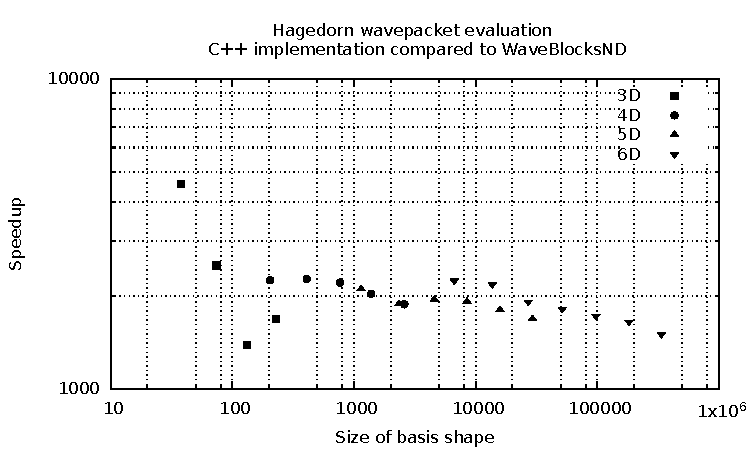
\includegraphics[width=1.0\textwidth]{plots/hawp_eval_cvp_fat}
  \caption{Wavepacket evaluation time in C++ compared to WaveBlocksND.
  WaveBlocksND uses the \textbf{fat recursion} routine.}
  \label{fig:hawp_eval_cvp_fat}
\end{figure}

\subsubsection{Gradient computation}

Below is a benchmark of the gradient computation. The employed wavepacket
has a limited hyperbolic cut basis shape\footnote{
  The cutoff limit is 100, sparsity varies between \(2^D\) and \(3^D\).}.
The results reveal run-time complexity improvements of my implementation.

\begin{figure}[H]
  \centering
  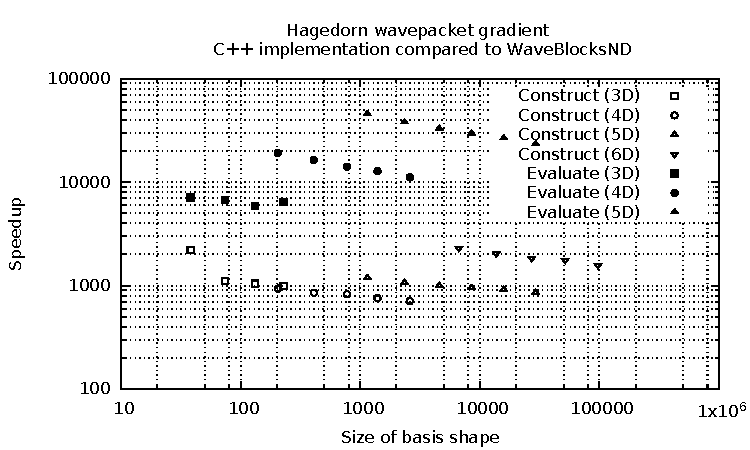
\includegraphics[width=1.0\textwidth]{plots/grad_eval_cvp}
  \caption{
    Wavepacket gradient construction and evaluation time in C++ compared to WaveBlocksND.
    Speedup means the run-time of WaveBlocksND divided by the run-time of my implementation.
    This chart contains two series: Empty bullets show the speedup when constructing
    the wavepacket gradient. Filled bullets show the speedup when evaluating the
    wavepacket gradient.
  }
  \label{fig:grad_eval_cvp}
\end{figure}

I've changed the way how shape extensions are generated. WaveBlocksND generates
shape extensions that contain many superfluous nodes. The ratio of superfluous to
essential nodes grows exponentially with the shape
dimensionality.\footnote{This effect is very apparent when using hyperbolic cut shapes.}
This results in a wavepacket gradient that has \(\mathcal{O}(\exp{}(D)\cdot N)\) basis functions instead of
\(\mathcal{O}(N)\).

WaveBlocksND mitigates this issue by constructing gradients using the scatter-type algorithm
since the scatter-type algorithm simply ignores superfluous nodes. This works well for low dimension.
Nevertheless the cost of allocating and zero-initialize oversized arrays
becomes apparent from dimensionality six (see \emph{construct}-series).

My implementation generates shape extensions that only contains essential nodes.
The \emph{evaluate}-series reflect the advantage of such minimal shape extensions
when evaluating wavepacket gradients.

\subsection{First steps towards parallelisation using OpenMP}

I paid attention to parallelisation right from the start.
The evaluation of Hagedorn wavepackets is of quite serial nature due to its
recursive scheme. However basis functions on the same slice can be evaluated independently.
This was one of my main reasons to split basis shapes into slices.
I added a simple \emph{pragma omp parallel for} to the loop that runs over all nodes
of the same slice. I've done some measurements on the Euler cluster using up to 12 threads.
The plot below (\ref{fig:hawp_eval_omp}) shows that the evaluation of large and high dimensional
wavepackets scales reasonable well.

\begin{figure}[H]
  \centering
  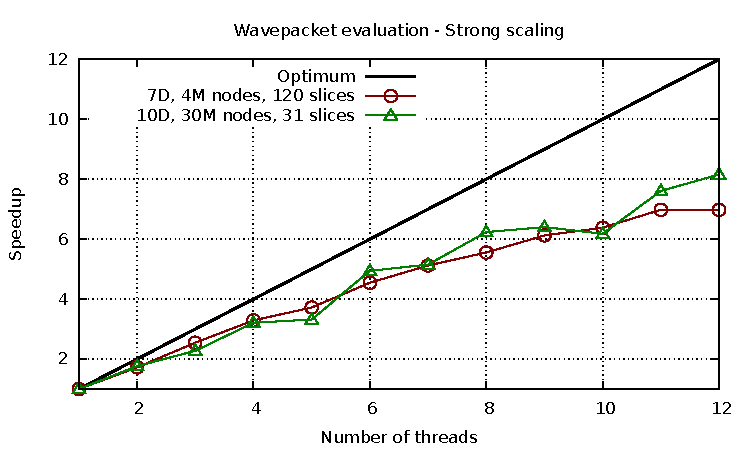
\includegraphics[width=1.0\textwidth]{plots/hawp_eval_omp}
  \caption{
    Strong scaling plot of the Hagedorn wavepacket evaluation.
    It shows two measurements of a 10-dimensional wavepackets
    with a basis shape of one million and 30 million nodes respectively.
  }
  \label{fig:hawp_eval_omp}
\end{figure}


\end{document}
